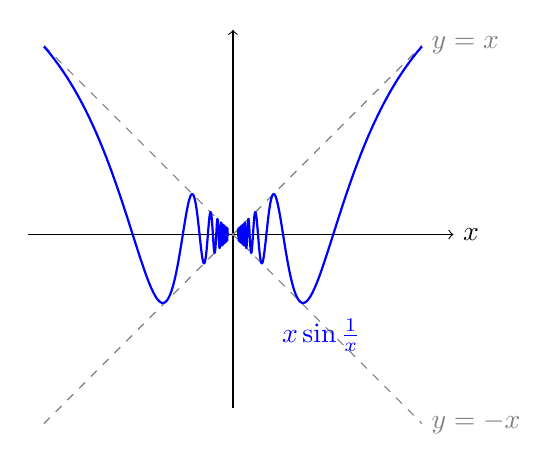
\begin{tikzpicture}[xscale=4, yscale=4]
  \draw[->] (-0.65,0) -- (0.7,0) node[right] {$x$};
  \draw[->] (0,-0.55) -- (0,0.65);
  \draw[gray, dashed] (-0.6,-0.6) -- (0.6,0.6) node[right] {$y=x$};
  \draw[gray, dashed] (-0.6,0.6) -- (0.6,-0.6) node[right] {$y=-x$};
  \draw[blue, thick, domain=1.667:60, samples=1500, variable=\u] plot ({1/\u}, {sin(deg(\u))/\u});
  \draw[blue, thick, domain=1.667:60, samples=1500, variable=\u] plot ({-1/\u}, {sin(deg(\u))/\u});
  \node[blue] at (0.28,-0.32) {$x\sin\frac1x$};
\end{tikzpicture}
